
\section{Алгоритм основного метода расчёта}
\label{sec:section8}
В этом заключительном разделе отчёта опишем, как в первой версии теплогидравлического кода реализован основной метод расчёта \texttt{Method\_1}, который выполняет очередной шаг по времени при расчёте теплогидравлической схемы.

Приведём окончательный вид полученных в других разделах настоящего отчёта дискретных аналогов уравнений сохранения и входящих в них коэффициентов:
\begin{itemize}[topsep=5pt, itemsep=-3pt]
\item уравнения сохранение массы и энергии для ячейки канала \eqref{formula518} и \eqref{formula513}
$$
\left(A_j^P \right)' \cdot \Delta(dG_{j}^n) + \left(B_j^P \right)' \cdot \Delta(dP_j^n) + \left(C_j^P \right)' \cdot \Delta(dG_{j+1}^n) = -\left(F_j^P \right)';
$$
$$
A_j^h \cdot \Delta(dG_{j}^n)+B_j^h \cdot \Delta(dh_j^n) + C_j^h \cdot \Delta(dG_{j+1}^n) + D_j^h \cdot \Delta(dP_j^n) = -F_j^h,
$$
где $\left(A_j^P \right)'=A_j^P - \frac{D_j^P}{B_j^h} \cdot A_j^h$;

\noindent \hspace{0.6cm} $\left(B_j^P \right)'=B_j^P - \frac{D_j^P}{B_j^h} \cdot D_j^h$;

\noindent \hspace{0.6cm} $\left(C_j^P \right)'=C_j^P - \frac{D_j^P}{B_j^h} \cdot C_j^h$;

\noindent \hspace{0.6cm} $\left(F_j^P \right)'=F_j^P - \frac{D_j^P}{B_j^h} \cdot F_j^h$,

\noindent где $A_j^P=-1$;

\noindent \hspace{0.6cm} $B_j^P=V \cdot f_{comp}\cdot \left( \frac{\partial\rho}{\partial P}\right)_{h} \cdot b_j^P$;

\noindent \hspace{0.6cm} $C_j^P=1$;

\noindent \hspace{0.6cm} $D_j^P=V \cdot f_{comp}\cdot \left(\frac{\partial\rho}{\partial h}\right)_{P} \cdot b_j^h$;

\noindent \hspace{0.6cm} $F_j^P=V\cdot f_{comp} \cdot \left(\left(\frac{\partial\rho}{\partial P}\right)_{h}\cdot \left(\frac{\partial P}{\partial\tau} \right) + \left(\frac{\partial\rho}{\partial h}\right)_{P}\cdot \left(\frac{\partial h}{\partial\tau} \right) \right) - G_j + G_{j+1}$;

\noindent \hspace{0.6cm} $\left(\frac{\partial P}{\partial\tau} \right)=a_j^P+b_j^P\cdot (P_j^{n+1}-P_j^{n \mathstrut})$; $\left(\frac{\partial h}{\partial\tau} \right)=a_j^h+b_j^h\cdot (h_j^{(n+1)}-h_j^{n \mathstrut})$;

\noindent \hspace{0.6cm} $A_j^h=-\mu_j\cdot (h_{j-1}-h_j)$;

\noindent \hspace{0.6cm} $B_j^h=\rho\cdot V\cdot b_j^h - min\left(\frac{\partial Q}{\partial h_j^n},0 \right)$;

\noindent \hspace{0.6cm} $C_j^h=(1-\mu_{j+1})\cdot (h_{j+1}-h_j)$;

\noindent \hspace{0.6cm} $D_j^h=-V \cdot b_j^P$;

\noindent \hspace{0.6cm} $F_j^h=\rho\cdot V\cdot\frac{\partial h}{\partial\tau}+A_j^h\cdot G_j + C_j^h\cdot G_{j+1}-V\cdot\frac{\partial P}{\partial\tau}-Q-min\left(\frac{\partial Q}{\partial h_j^n},0 \right)\cdot dh_j^n$;

\item уравнение сохранения импульса для гидравлической связи \eqref{formula511}
$$
A_j^G \cdot \Delta(dP_{j-1}^n)+B_j^G \cdot \Delta(dG_j^n) + C_j^G \cdot \Delta(dP_j^n) = -F_j^G, 
$$
где $A_j^G=-1$; 

\noindent \hspace{0.6cm} $B_j^G = J_j \cdot b_j^G + F_{fr}^n\cdot | G_j^n | - min\left(\frac{\partial H_{pump}}{\partial G_j},0\right)$;

\noindent \hspace{0.6cm} $C_j^G=1$;

\noindent \hspace{0.6cm} $F_j^G=J_j \cdot \frac{\partial G_j}{\partial\tau} - P_{j-1} + P_j + \Delta P_{fr} + \Delta P_{acc} + \Delta P_{niv} - \Delta P_{pump} - min\left(\frac{\partial P_{pump}}{\partial G_j},0\right)\cdot dG_j^n$,

\noindent где $\Delta P_{fr}=F_{fr}^n\cdot | G_j^n | \cdot G_j^{n+1}$;

\noindent \hspace{0.6cm} $F_{fr}^n=\left[\left(\frac{\lambda\cdot\frac L 2}{d_g} + \xi \right)\cdot \frac{1}{2\cdot\rho\cdot S^2} \right]_{in} + \left[\left(\frac{\lambda\cdot\frac L 2}{d_g} + \xi \right)\cdot \frac{1}{2\cdot\rho\cdot S^2} \right]_{out}$;

\noindent \hspace{0.6cm} $\Delta P_{acc}$ --- определяется по соответствующим справочным формулам для однофазного или двухфазного потока по параметрам в соседних с гидравлической связью расчётных ячейках;

\noindent \hspace{0.6cm} $\Delta P_{niv}=\rho_{j-1}^n\cdot g \cdot \frac{\Delta Z_{j-1}}{2}+\rho_{j}^n\cdot g \cdot \frac{\Delta Z_{j}}{2}$;

\item уравнение сохранения энергии для контрольного объёма (\eqref{formula513} совместно с \eqref{formula417})  
$$
\sum_{k=1}^{N_{in}} A_{kj}^h \cdot \Delta(dG_{j,in}^n)+B_j^h \cdot \Delta(dh_j^n) + \sum_{k=1}^{N_{out}} C_{kj}^h \cdot \Delta(dG_{j,out}^n) + D_j^h \cdot \Delta(dP_j^n) = -F_j^h,
$$
где $A_{kj}^h=-\mu_k\cdot (h_k-h_j)$;

\noindent \hspace{0.6cm} $B_j^h=\rho\cdot V\cdot b_j^h - min\left(\frac{\partial Q}{\partial h_j^n},0 \right)$;

\noindent \hspace{0.6cm} $C_{kj}^h=(1-\mu_k)\cdot (h_k-h_j)$;

\noindent \hspace{0.6cm} $D_j^h=-V \cdot b_j^P$; 

\item уравнение для связи давлений в трёх соседних ячейках канала \eqref{formula65}
$$
\left(A_j^P \right)'' \cdot \Delta(dP_{j-1}^n) + \left(B_j^P \right)'' \cdot \Delta(dP_j^n) + \left(C_j^P \right)'' \cdot \Delta(dP_{j+1}^n) = -\left(F_j^P \right)'',
$$
где $\left(A_j^P \right)''=-\left(A_j^P \right)' \cdot \frac{A_j^G}{B_j^G}$;

\noindent \hspace{0.6cm} $\left(B_j^P \right)''=\left(B_j^P \right)'-\left(A_j^P \right)' \cdot \frac{C_j^G}{B_j^G} - \left(C_j^P \right)'\cdot \frac{A_{j+1}^G}{B_{j+1}^G}$;

\noindent \hspace{0.6cm} $\left(C_j^P \right)''=- \left(C_j^P \right)'\cdot \frac{C_{j+1}^G}{B_{j+1}^G}$;

\noindent \hspace{0.6cm} $\left(F_j^P \right)''=\left(F_j^P \right)' - \frac{\left(A_j^P \right)'}{B_j^G}\cdot F_j^G - \frac{\left(C_j^P \right)'}{B_{j+1}^G}\cdot F_{j+1}^G$;

\item уравнение для связи энтальпий в трёх соседних ячейках канала \eqref{formula75}
$$
A_j^h \cdot \Delta(dh_{j-1}^n) + B_j^h \cdot \Delta(dh_j^n) + C_j^h \cdot \Delta(dh_{j+1}^n)  = -F_j^h,
$$
где $A_j^h=- \mu_j \cdot G_j^{n+1}$;

\noindent \hspace{0.6cm} $C_j^h = (1-\mu_{j+1}) \cdot G_{j+1}^{n+1}$;

\noindent \hspace{0.6cm} $B_j^h = \rho \cdot V \cdot b_j^h - min\left(\frac{\partial Q}{\partial h_j^n},0 \right)-A_j^h-C_j^h$;

\noindent \hspace{0.6cm} $F_j^h = \rho\cdot V\cdot\frac{\partial h}{\partial\tau}+A_j^h\cdot (h_{j-1}-h_j) + C_j^h\cdot (h_{j+1}-h_j)-V\cdot\frac{\partial P}{\partial\tau}-Q-min\left(\frac{\partial Q}{\partial h_j^n},0 \right)\cdot dh_j^n$;

\item уравнение для давления в узле (уравнение сохранения массы для узла) \eqref{formula631}
$$
\sum_{j=1}^{N_{in}} \left(A_k^P \right)_j^{*} \cdot \Delta \left(dP_{u_{in}}^n \right)_j + \left(B_k^P \right)^{*} \cdot \Delta \left(dP_u^n \right) + \sum_{j=1}^{N_{out}} \left(C_k^P \right)_j^{*} \cdot \Delta \left(dP_{u_{out}}^n \right)_j = -\left(F_k^P \right)^{*},
$$
где $\left(A_k^P \right)_j^{*}=\left(A_k^P \right)' \cdot \frac{1}{(B_N^G)_j}\cdot\left[-(A_N^G)_j(S_{N-1}^1)_j\right]$;

\noindent \hspace{0.6cm} $\left(B_k^P \right)^{*}=\left(B_k^P \right)'+\left(A_k^P \right)'\cdot \sum_{j=1}^{N_{in}} \frac{-1}{(B_N^G)_j}\cdot[(A_N^G)_j(S_{N-1}^2)_j+(C_N^G)_j] + \left(C_k^P \right)'\cdot \sum_{j=1}^{N_{out}} \frac{-1}{(B_0^G)_j}\cdot [(A_0^G)_j+(C_0^G)_j(S_0^1)_j]$;

\noindent \hspace{0.6cm} $\left(C_k^P \right)_j^{*}=\left(C_k^P \right)' \cdot \frac{1}{(B_0^G)_j}\cdot\left[-(C_0^G)_j(S_0^2)_j\right]$;

\noindent \hspace{0.6cm} $\left(F_k^P \right)^{*}=\left(F_k^P \right)'-\left(A_k^P \right)'\cdot \sum_{j=1}^{N_{in}} \frac{1}{(B_N^G)_j}\cdot[(F_N^G)_j+(A_N^G)_j(S_{N-1}^0)_j] - \left(C_k^P \right)'\cdot \sum_{j=1}^{N_{out}} \frac{1}{(B_0^G)_j}\cdot [(F_0^G)_j+(C_0^G)_j(S_0^0)_j] $,

\noindent где $N_{in}$ --- количество рёбер, входящих в рассматриваемый узел; $N_{out}$ --- количество рёбер, выходящих из рассматриваемого узла, $k$ --- индекс рассматриваемого узла; $S^0$, $S^1$ и $S^2$ --- коэффициенты в выражении давления в ячейке канала через давления в ограничивающих этот канал узлах (уравнение \eqref{formula623});

\item уравнение для энтальпии в узле (уравнение сохранения энергии для узла) \eqref{formula714}
$$
\sum_{j=1}^{N_{in}} (A_j^h)^{*} \cdot \Delta(dh_j^n) + (B_k^h)^{*} \cdot \Delta(dh_k^n) + \sum_{j=1}^{N_{out}} (C_j^h)^{*} \cdot \Delta(dh_j^n) = -(F_k^h)^{*}, 
$$
где $(A_j^h)^{*} = A_j^h \cdot (S_{N-1}^1)_j$;

\noindent \hspace{0.6cm} $(B_k^h)^{*} = B_k^h + \sum_{j=1}^{N_{in}} A_j^h \cdot (S_{N-1}^2)_j + \sum_{j=1}^{N_{out}} C_j^h \cdot (S_0^1)_j$;

\noindent \hspace{0.6cm} $(C_j^h)^{*} = C_j^h \cdot (S_0^2)_j$; 

\noindent \hspace{0.6cm} $(F_k^h)^{*} = F_k^h+\sum_{j=1}^{N_{in}} A_j^h \cdot (S_{N-1}^0)_j + \sum_{j=1}^{N_{out}} C_j^h \cdot (S_0^0)_j$,

\noindent где $S^0$, $S^1$ и $S^2$ --- коэффициенты в выражении энтальпии в ячейке канала через энтальпии в ограничивающих этот канал узлах (уравнение \eqref{formula76}).  

\end{itemize}

На рисунках \ref{fig91} -- \ref{fig97} приведена блок-схема алгоритм метода выполнения шага расчёта с достаточно подробными комменариями. 
Отметим, что при определении, достигнута ли достаточная точность решения для перехода на следующих шаг по времени, используется сравнение прогнозного решения и фактически найденного. Если отличие этих двух решений велико, то это означает, что в пределах шага по времени произошли какие-то существенные изменения параметров, и поэтому шаг интегрирования следует уменьшить, а затем повторить решение с меньшим шагом. 
\begin{figure}
\abovecaptionskip=2pt
\centering{
	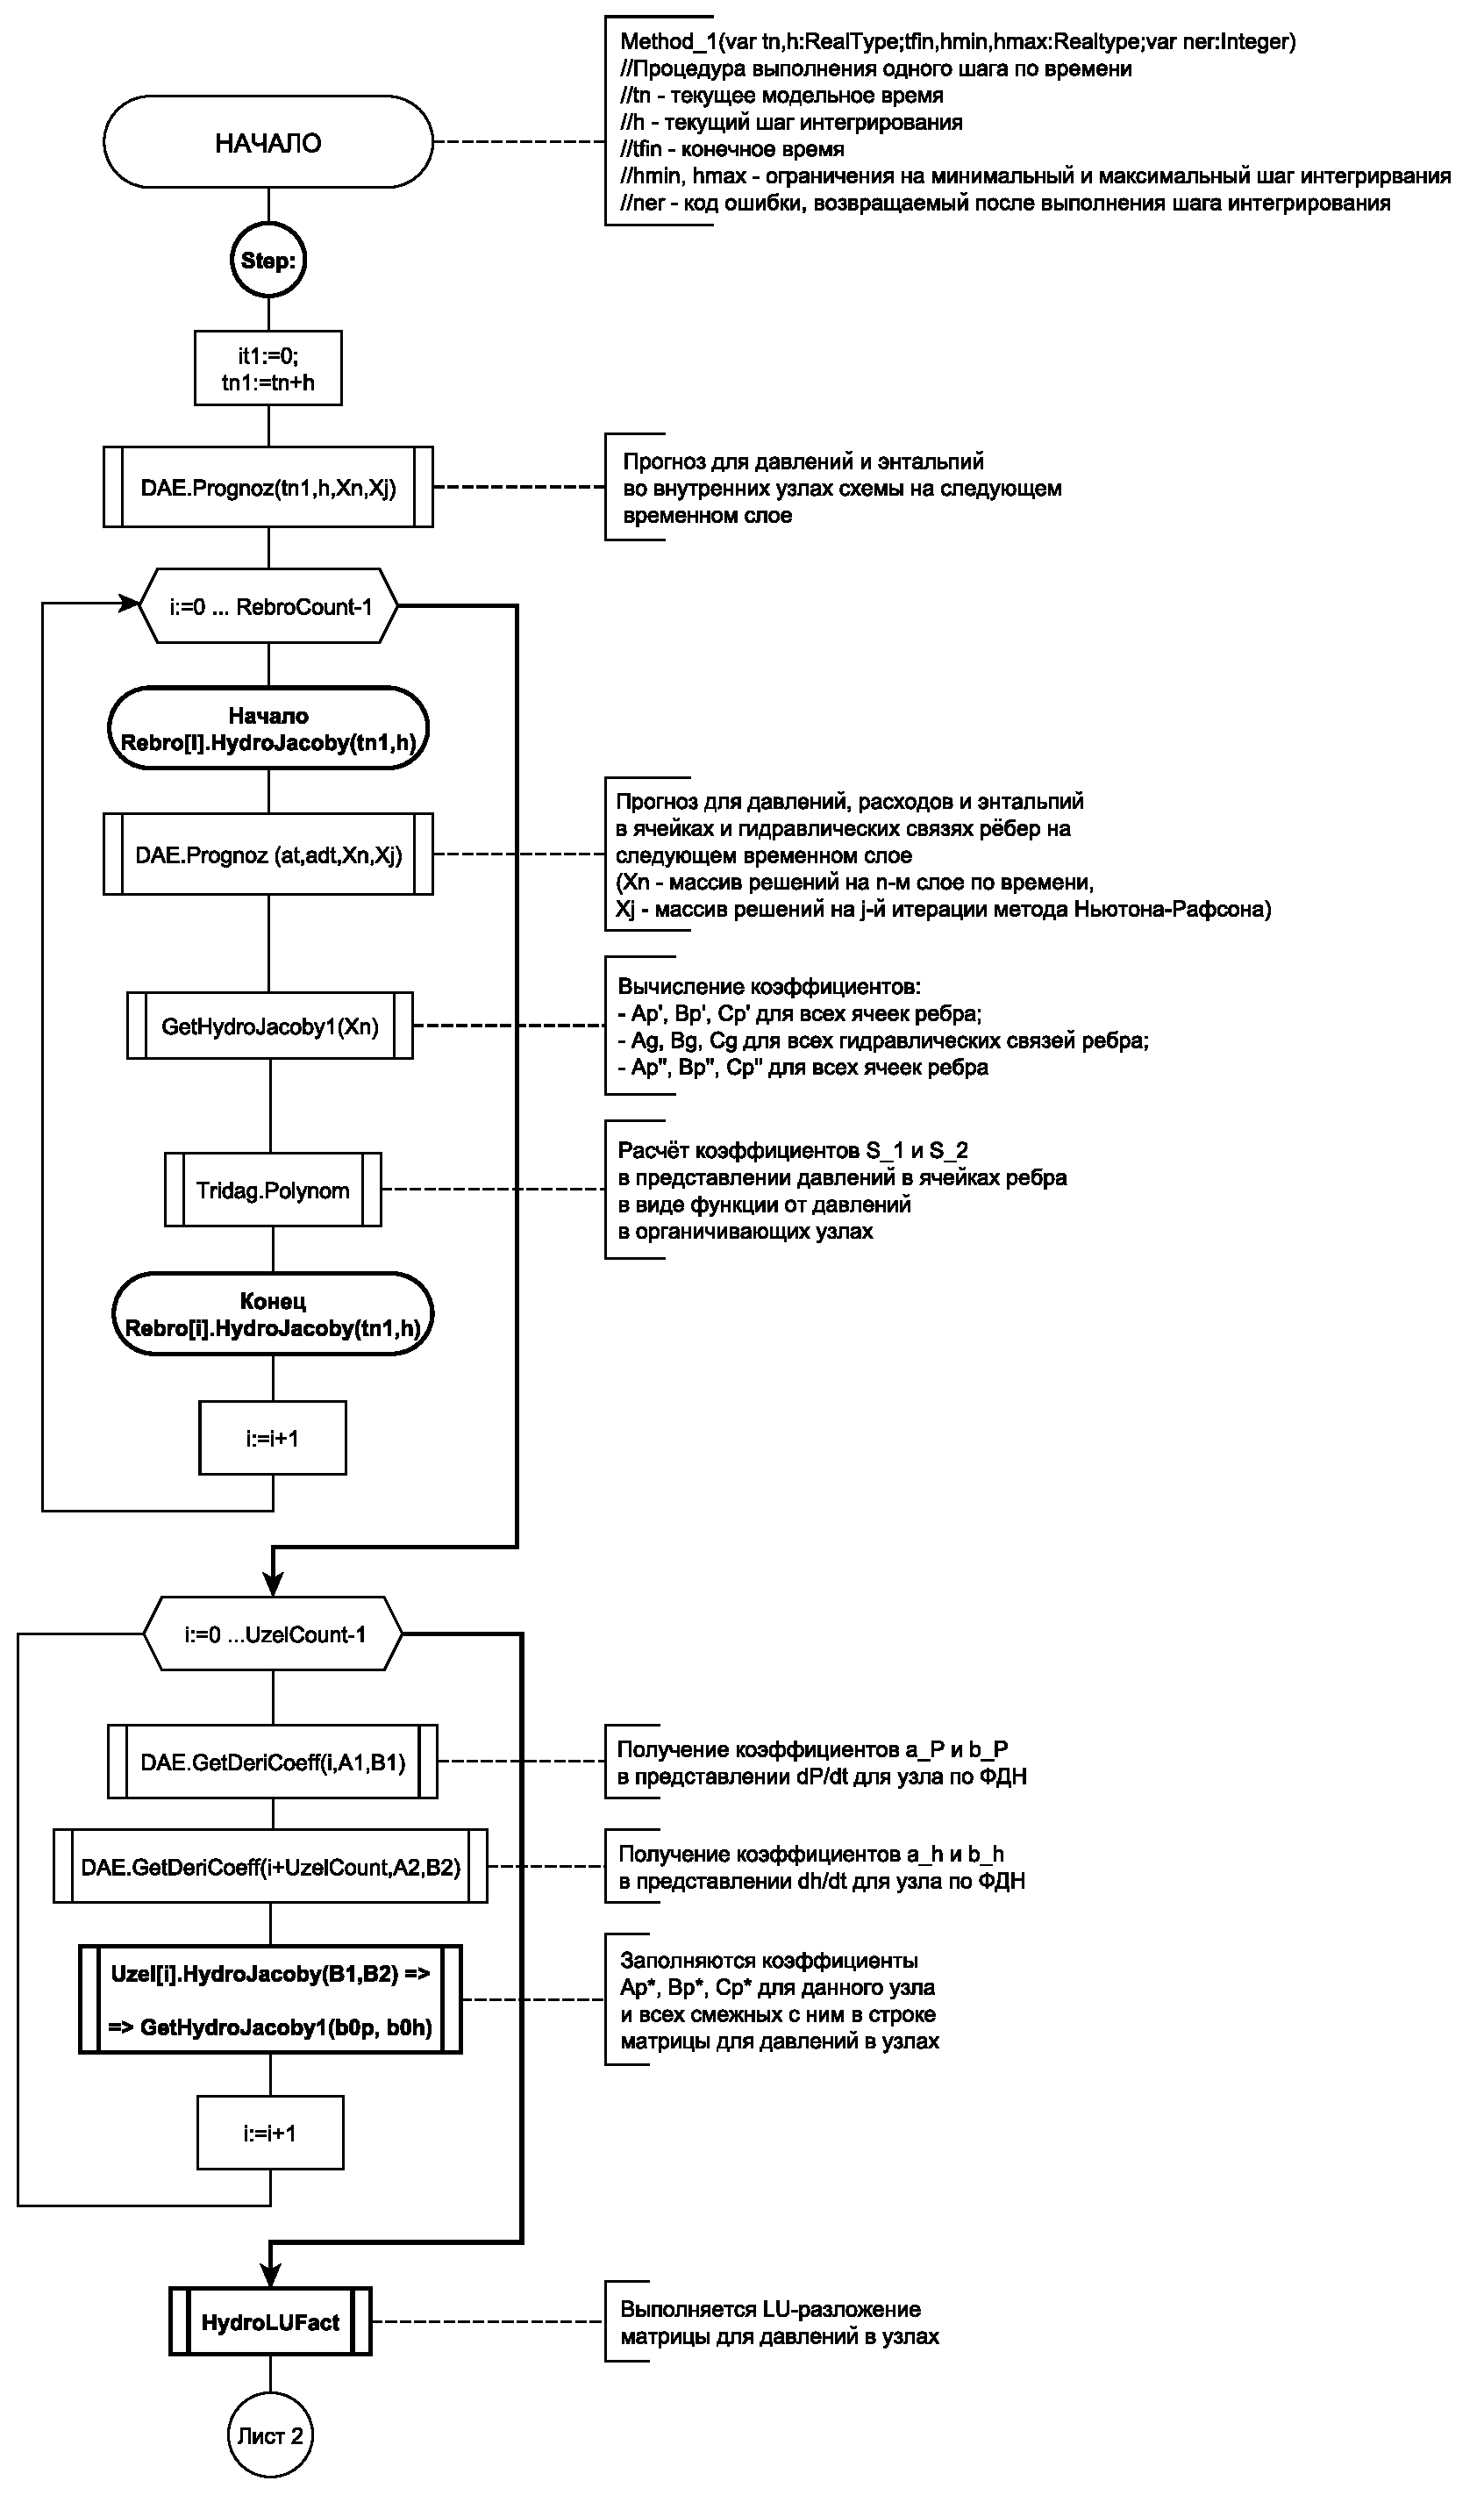
\includegraphics[width=0.89\linewidth]{Block_Scheme_Method1_List1.eps} 
	\caption{\textsc{Блок--схема алгоритма выполнения шага расчёта (лист 1)}}\label{fig91}
}
\end{figure}
\begin{figure}
\centering{
	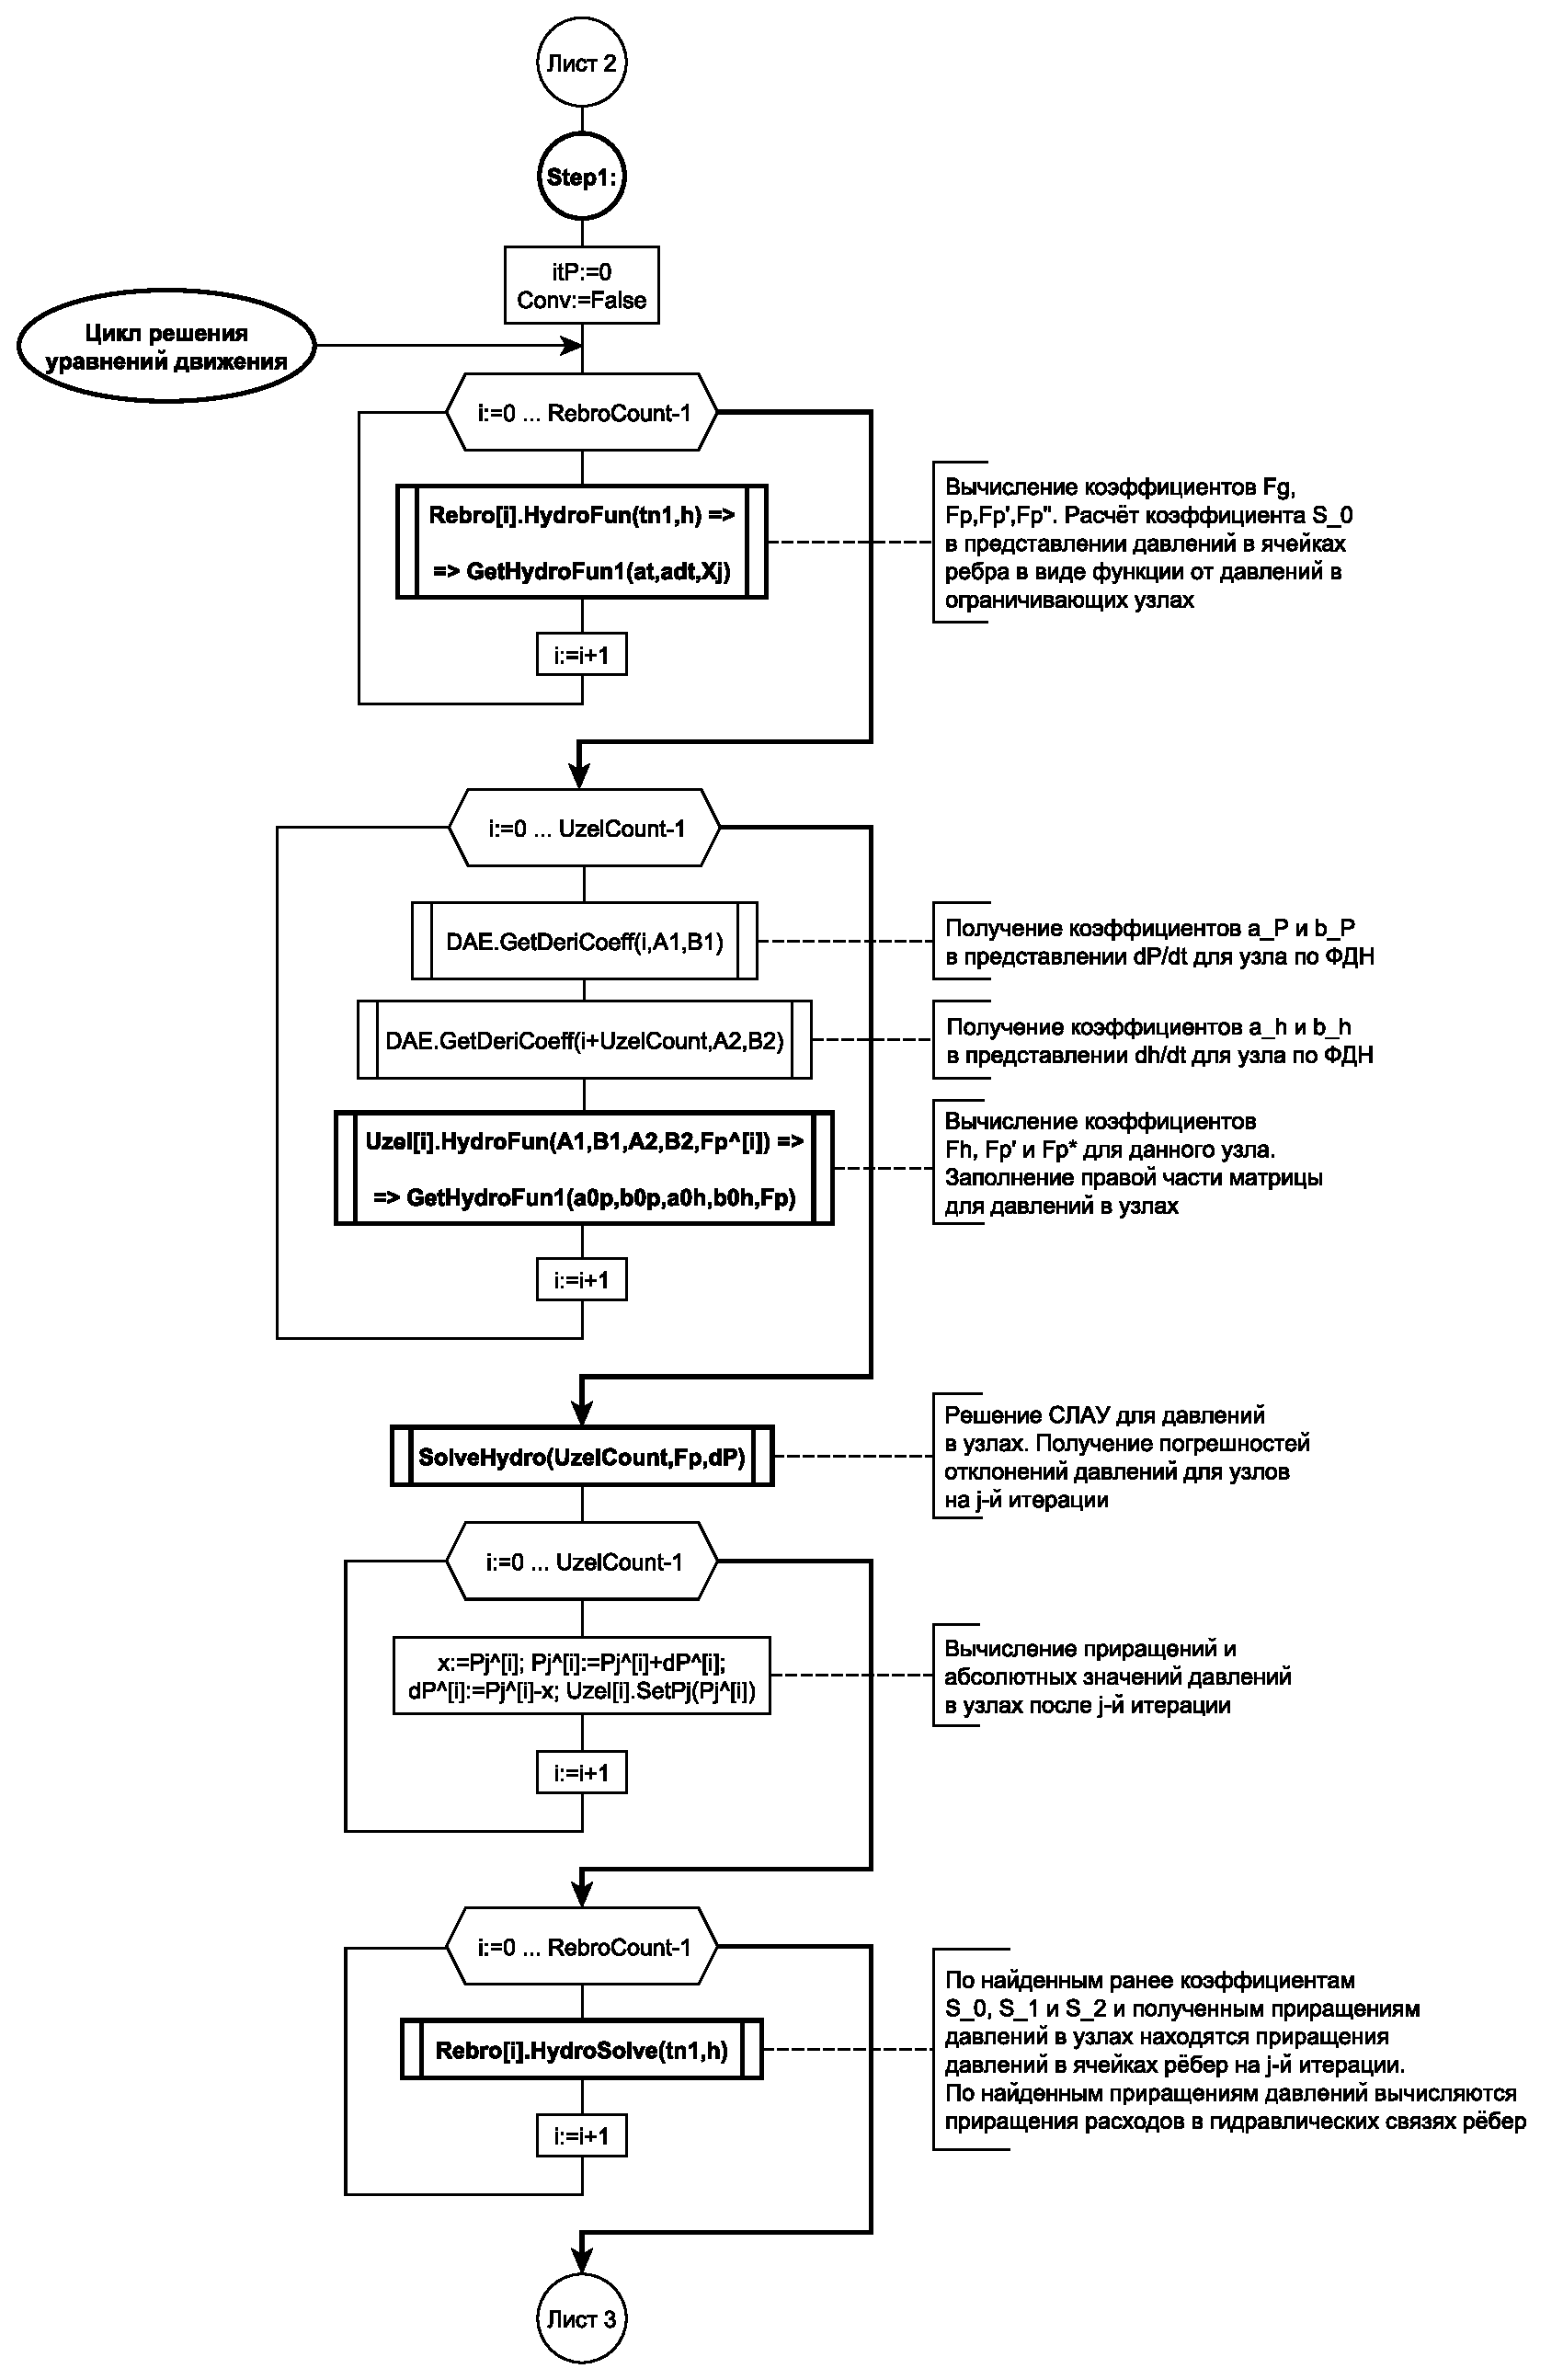
\includegraphics[width=0.97\linewidth]{Block_Scheme_Method1_List2.eps} 
	\caption{\textsc{Блок--схема алгоритма выполнения шага расчёта (лист 2)}}\label{fig92}
}
\end{figure}
\begin{figure}
\centering{
	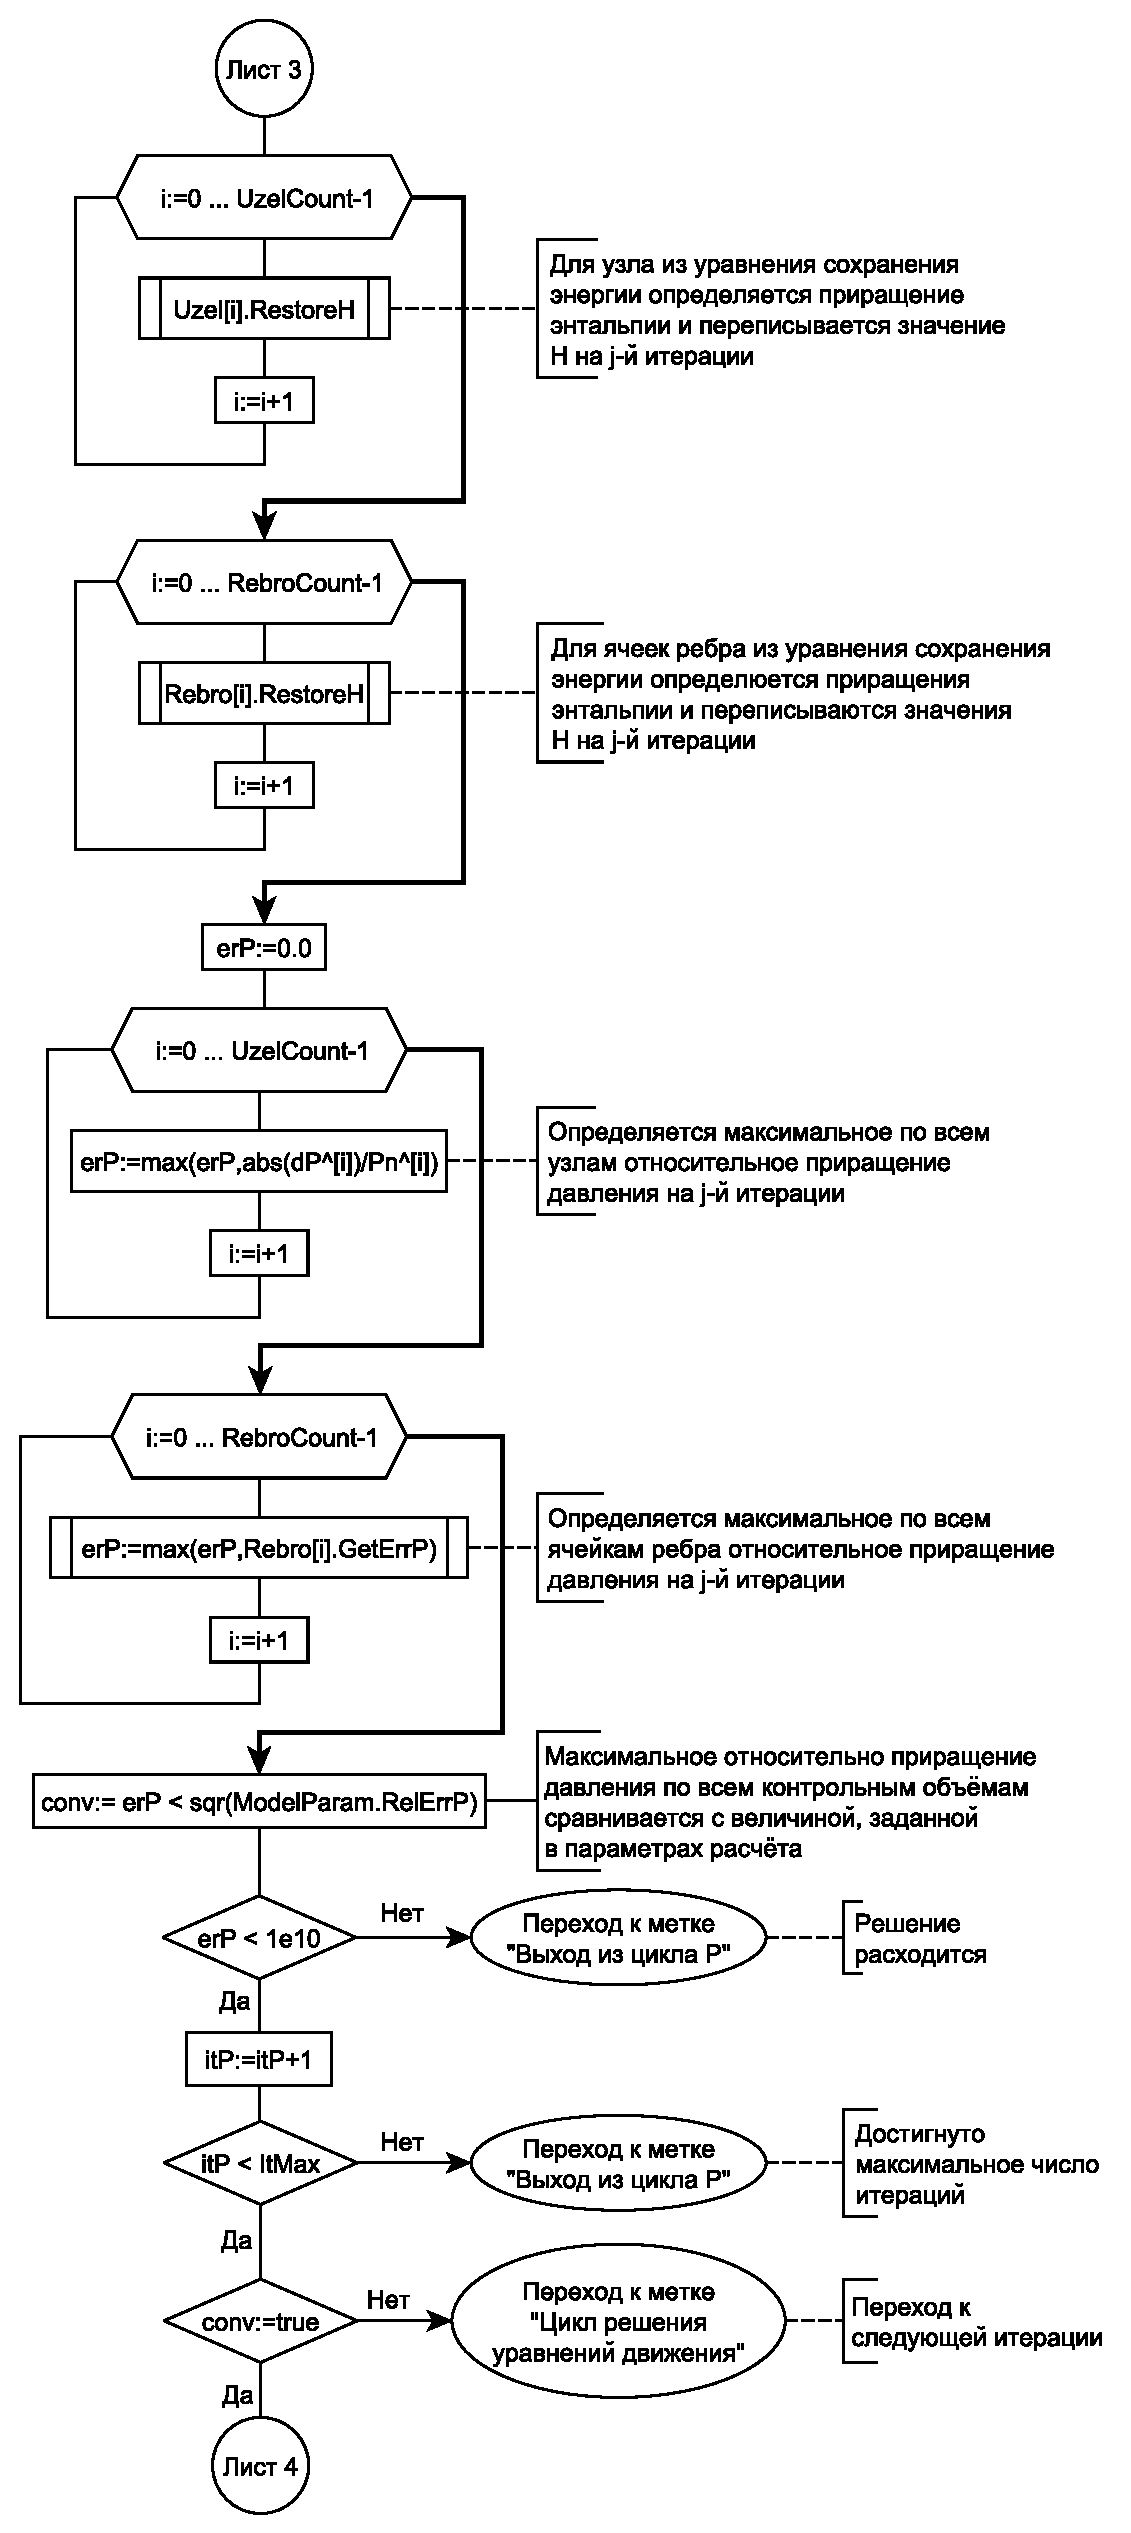
\includegraphics[width=0.65\linewidth]{Block_Scheme_Method1_List3.eps} 
	\caption{\textsc{Блок--схема алгоритма выполнения шага расчёта (лист 3)}}\label{fig93}
}
\end{figure}
\begin{figure}
\centering{
	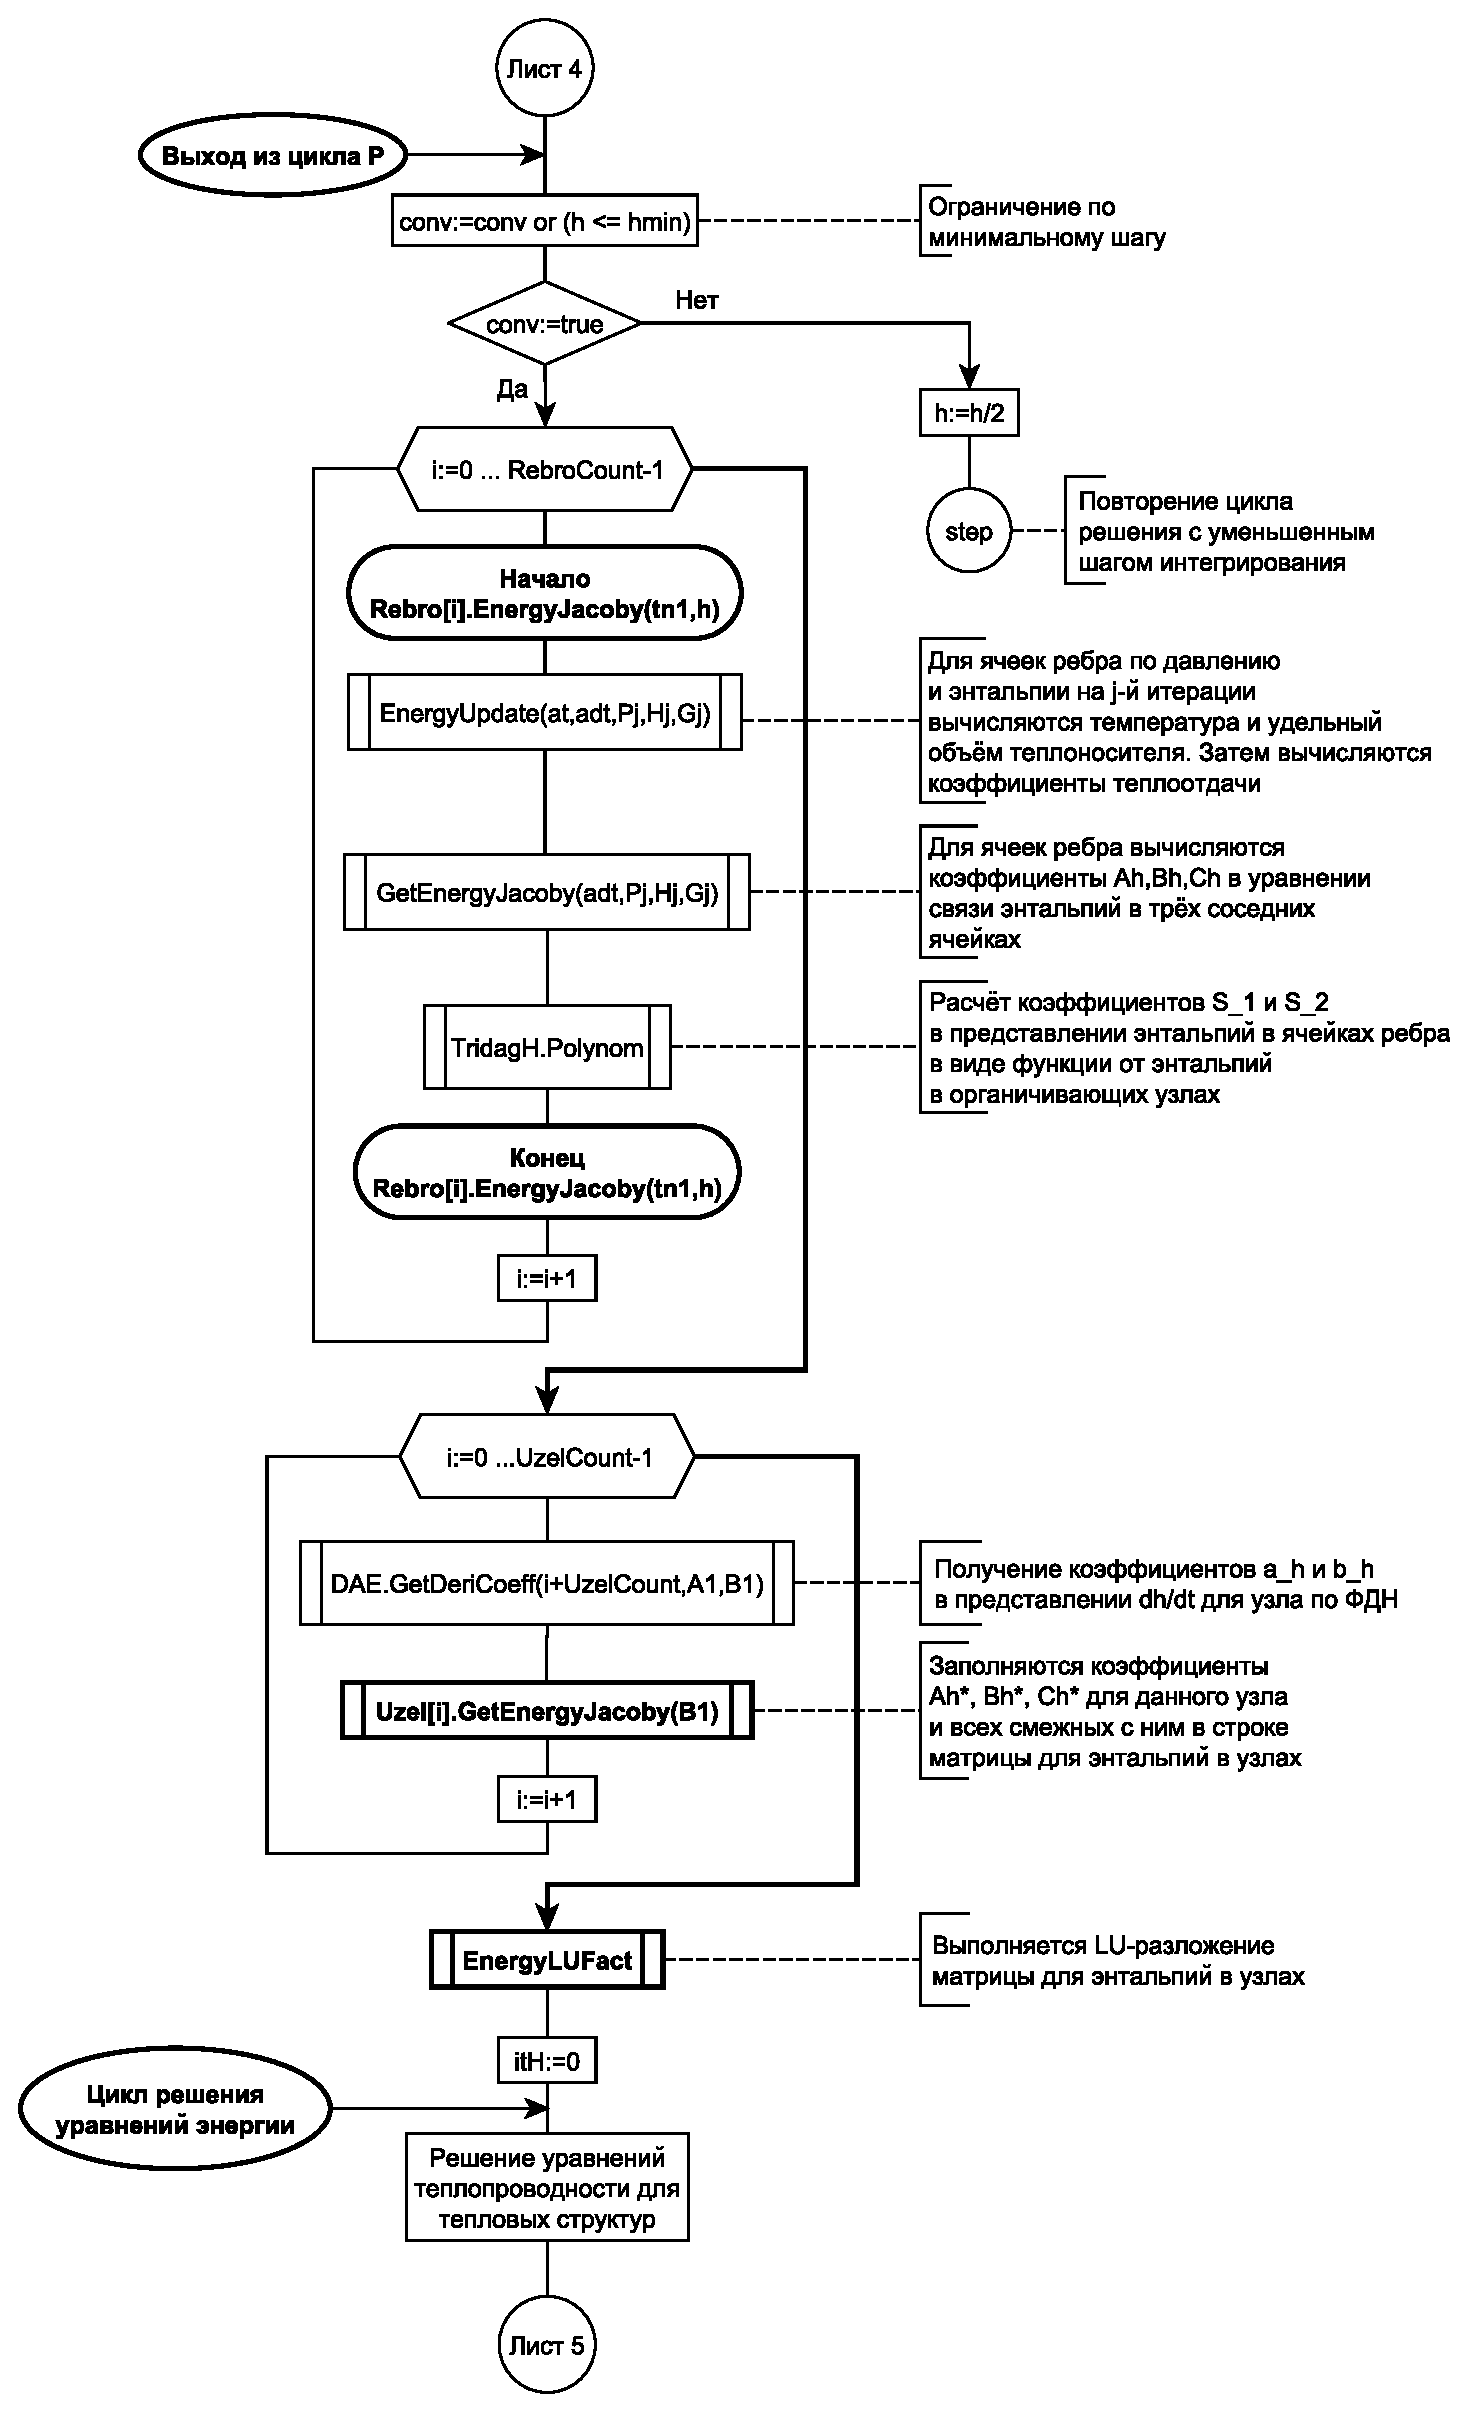
\includegraphics[width=0.91\linewidth]{Block_Scheme_Method1_List4.eps} 
	\caption{\textsc{Блок--схема алгоритма выполнения шага расчёта (лист 4)}}\label{fig94}
}
\end{figure}
\begin{figure}
\centering{
	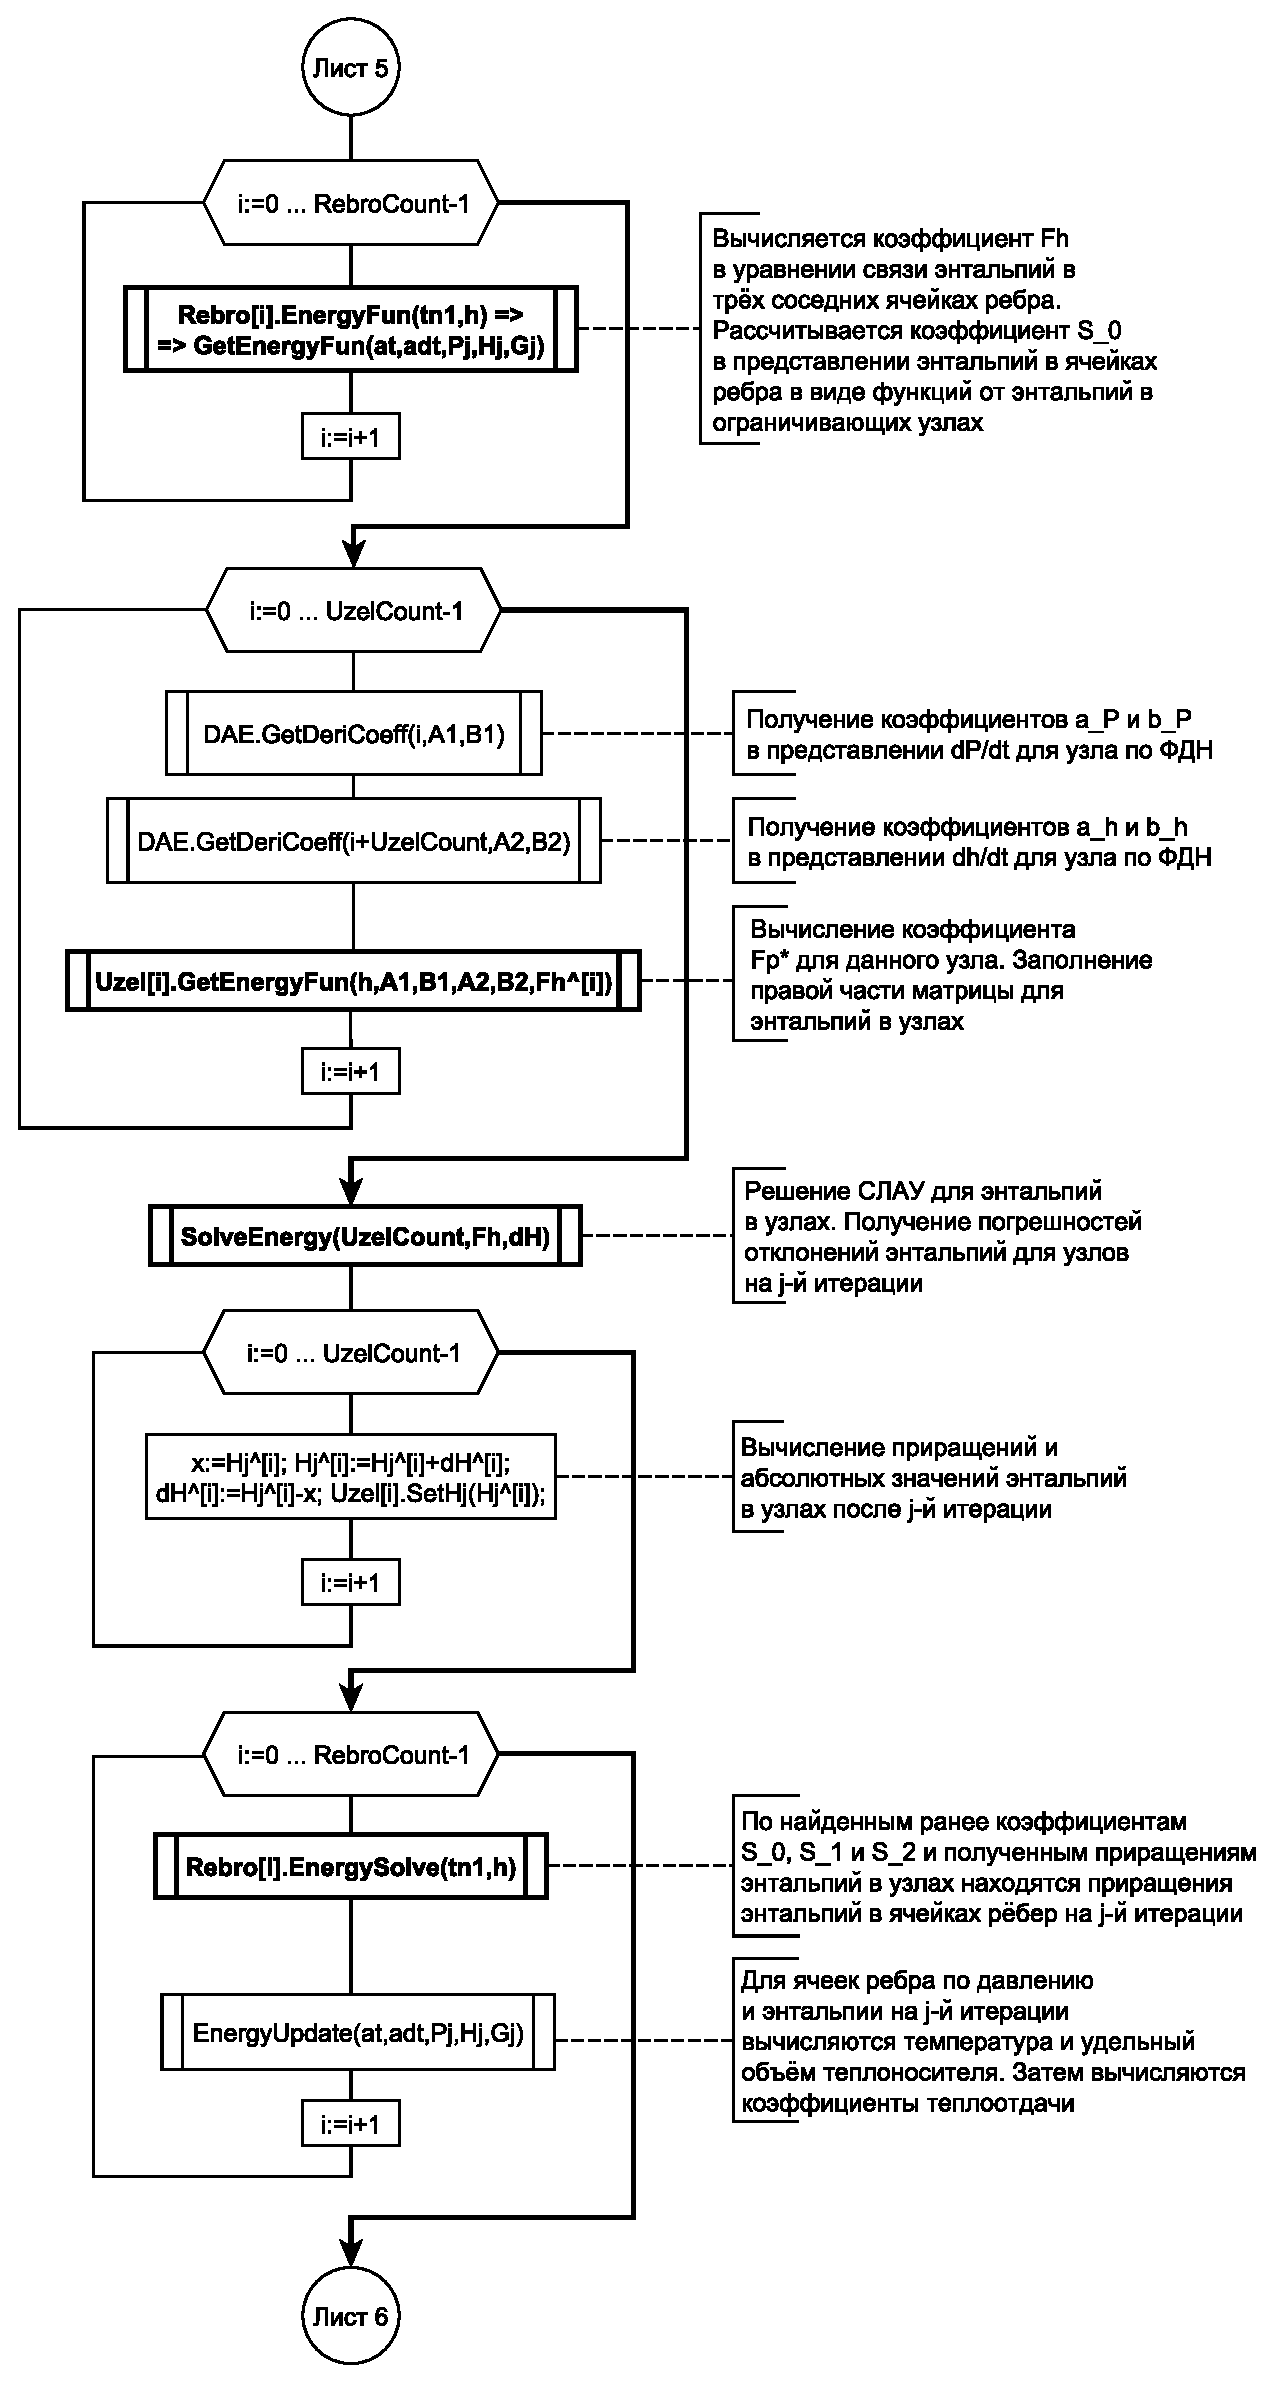
\includegraphics[width=0.79\linewidth]{Block_Scheme_Method1_List5.eps} 
	\caption{\textsc{Блок--схема алгоритма выполнения шага расчёта (лист 5)}}\label{fig95}
}
\end{figure}
\begin{figure}
\centering{
	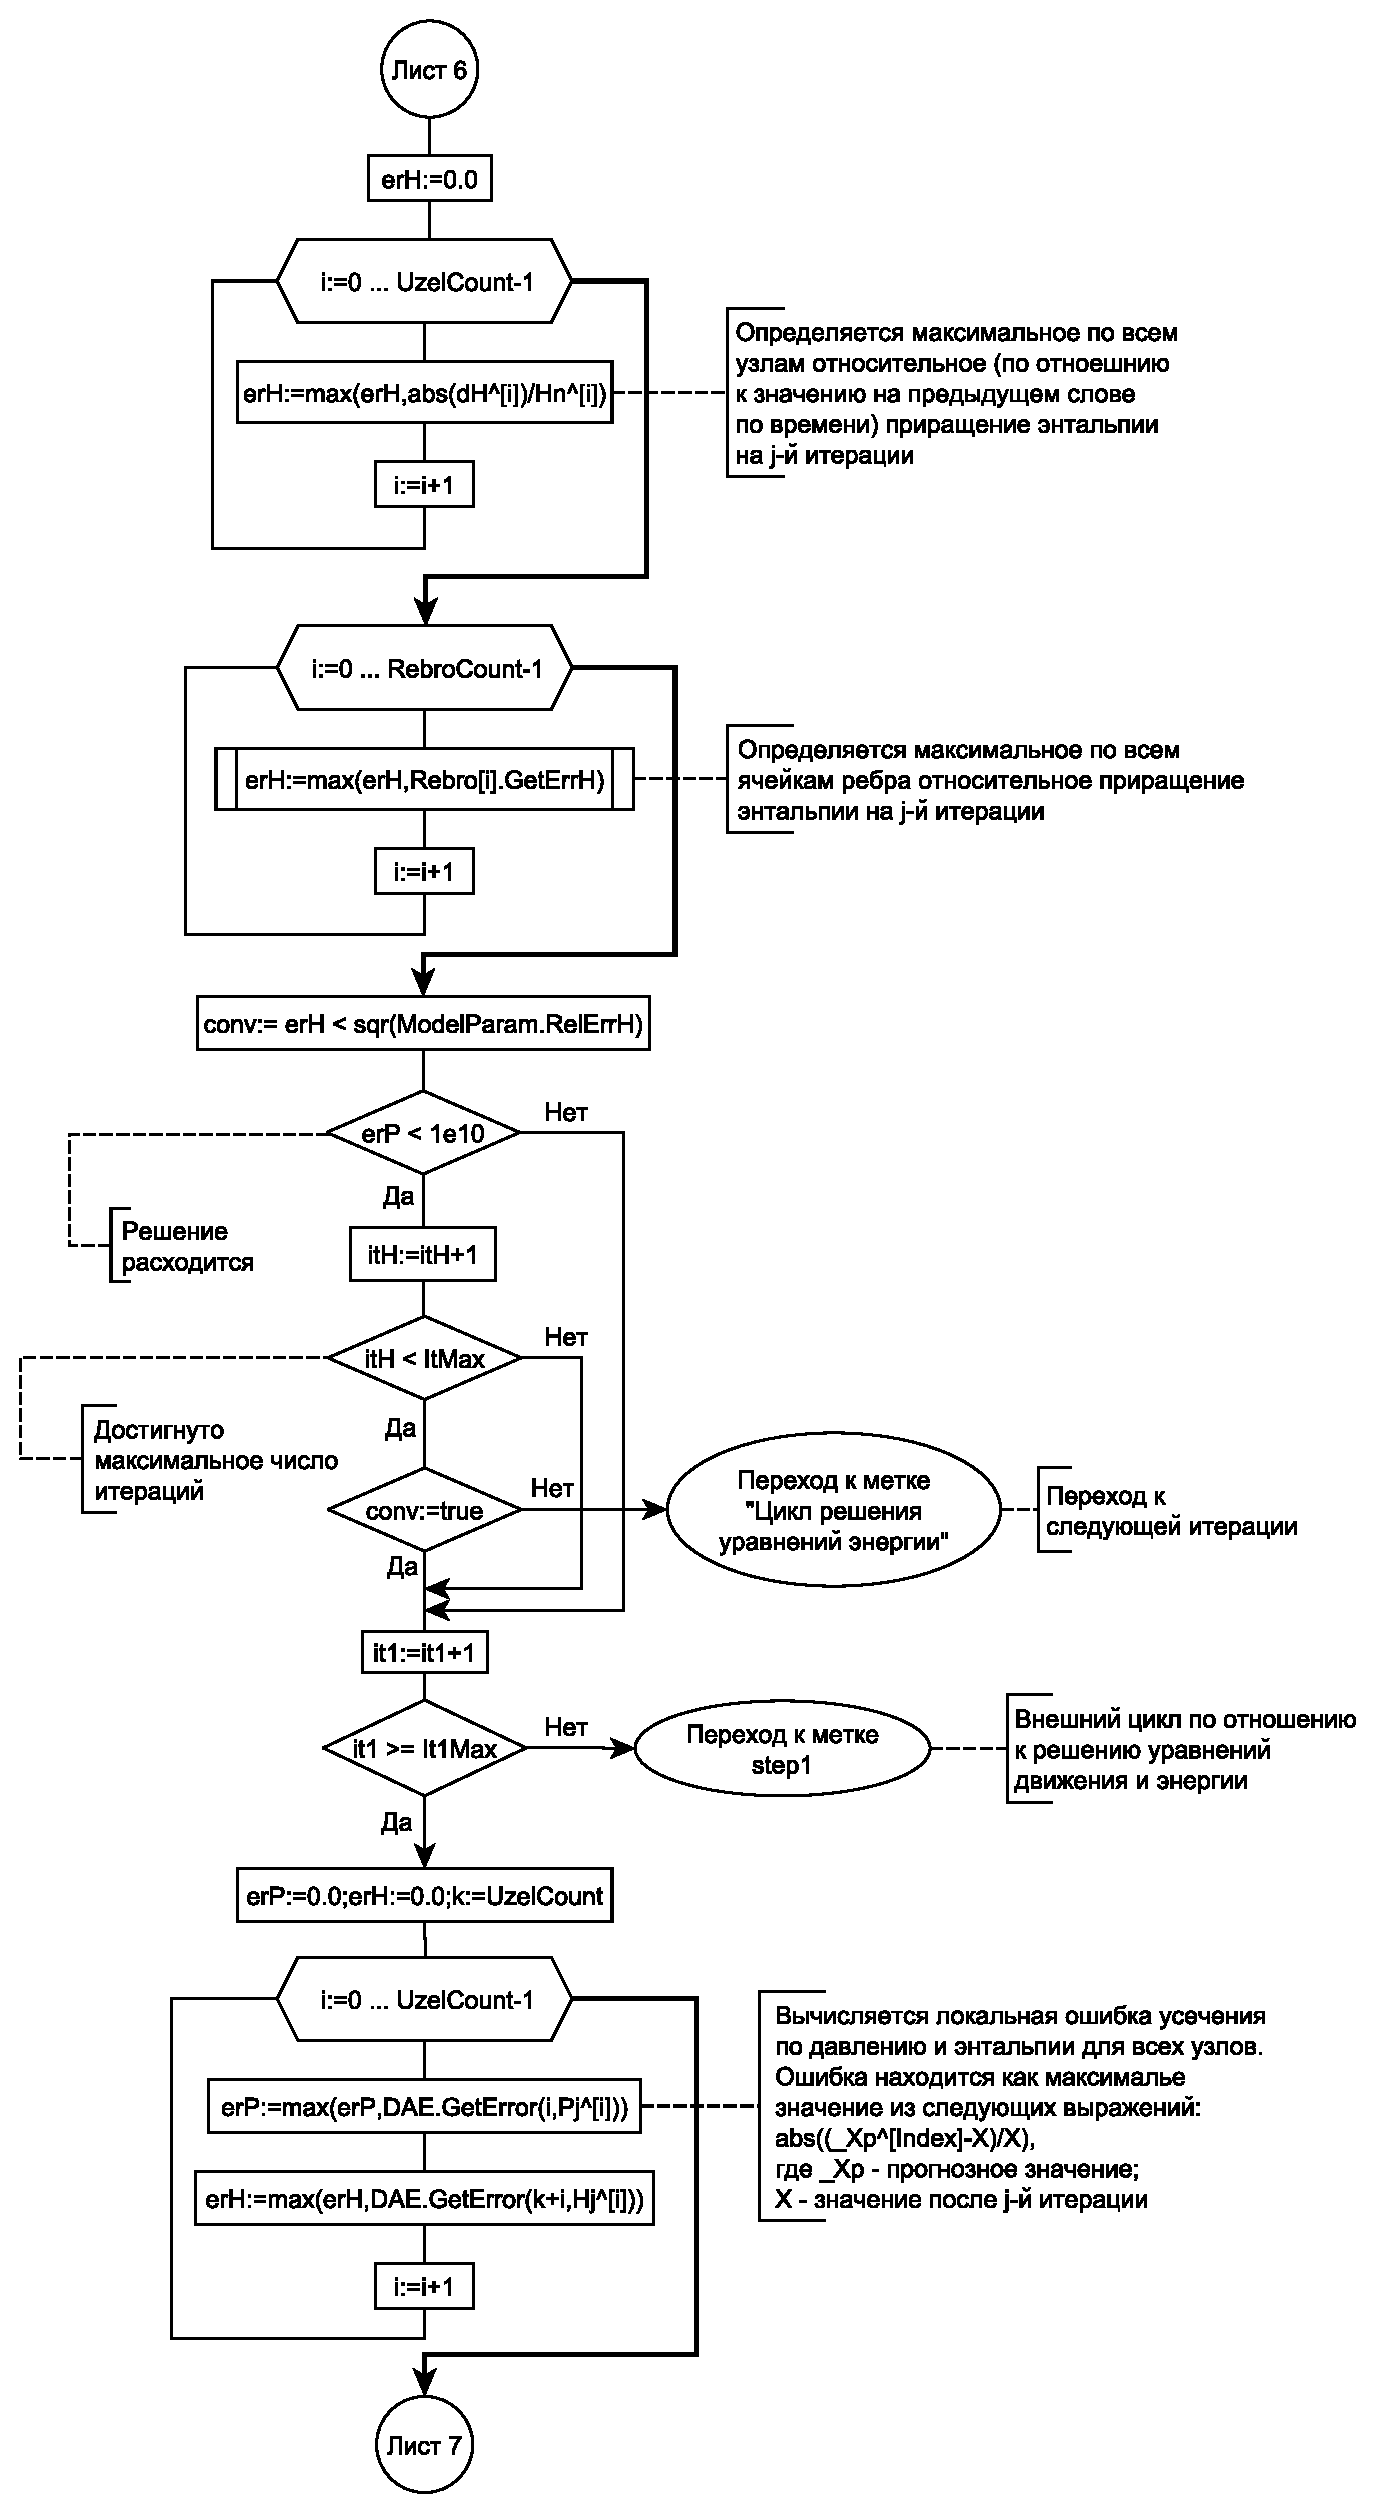
\includegraphics[width=0.72\linewidth]{Block_Scheme_Method1_List6.eps} 
	\caption{\textsc{Блок--схема алгоритма выполнения шага расчёта (лист 6)}}\label{fig96}
}
\end{figure}
\begin{figure}
\centering{
	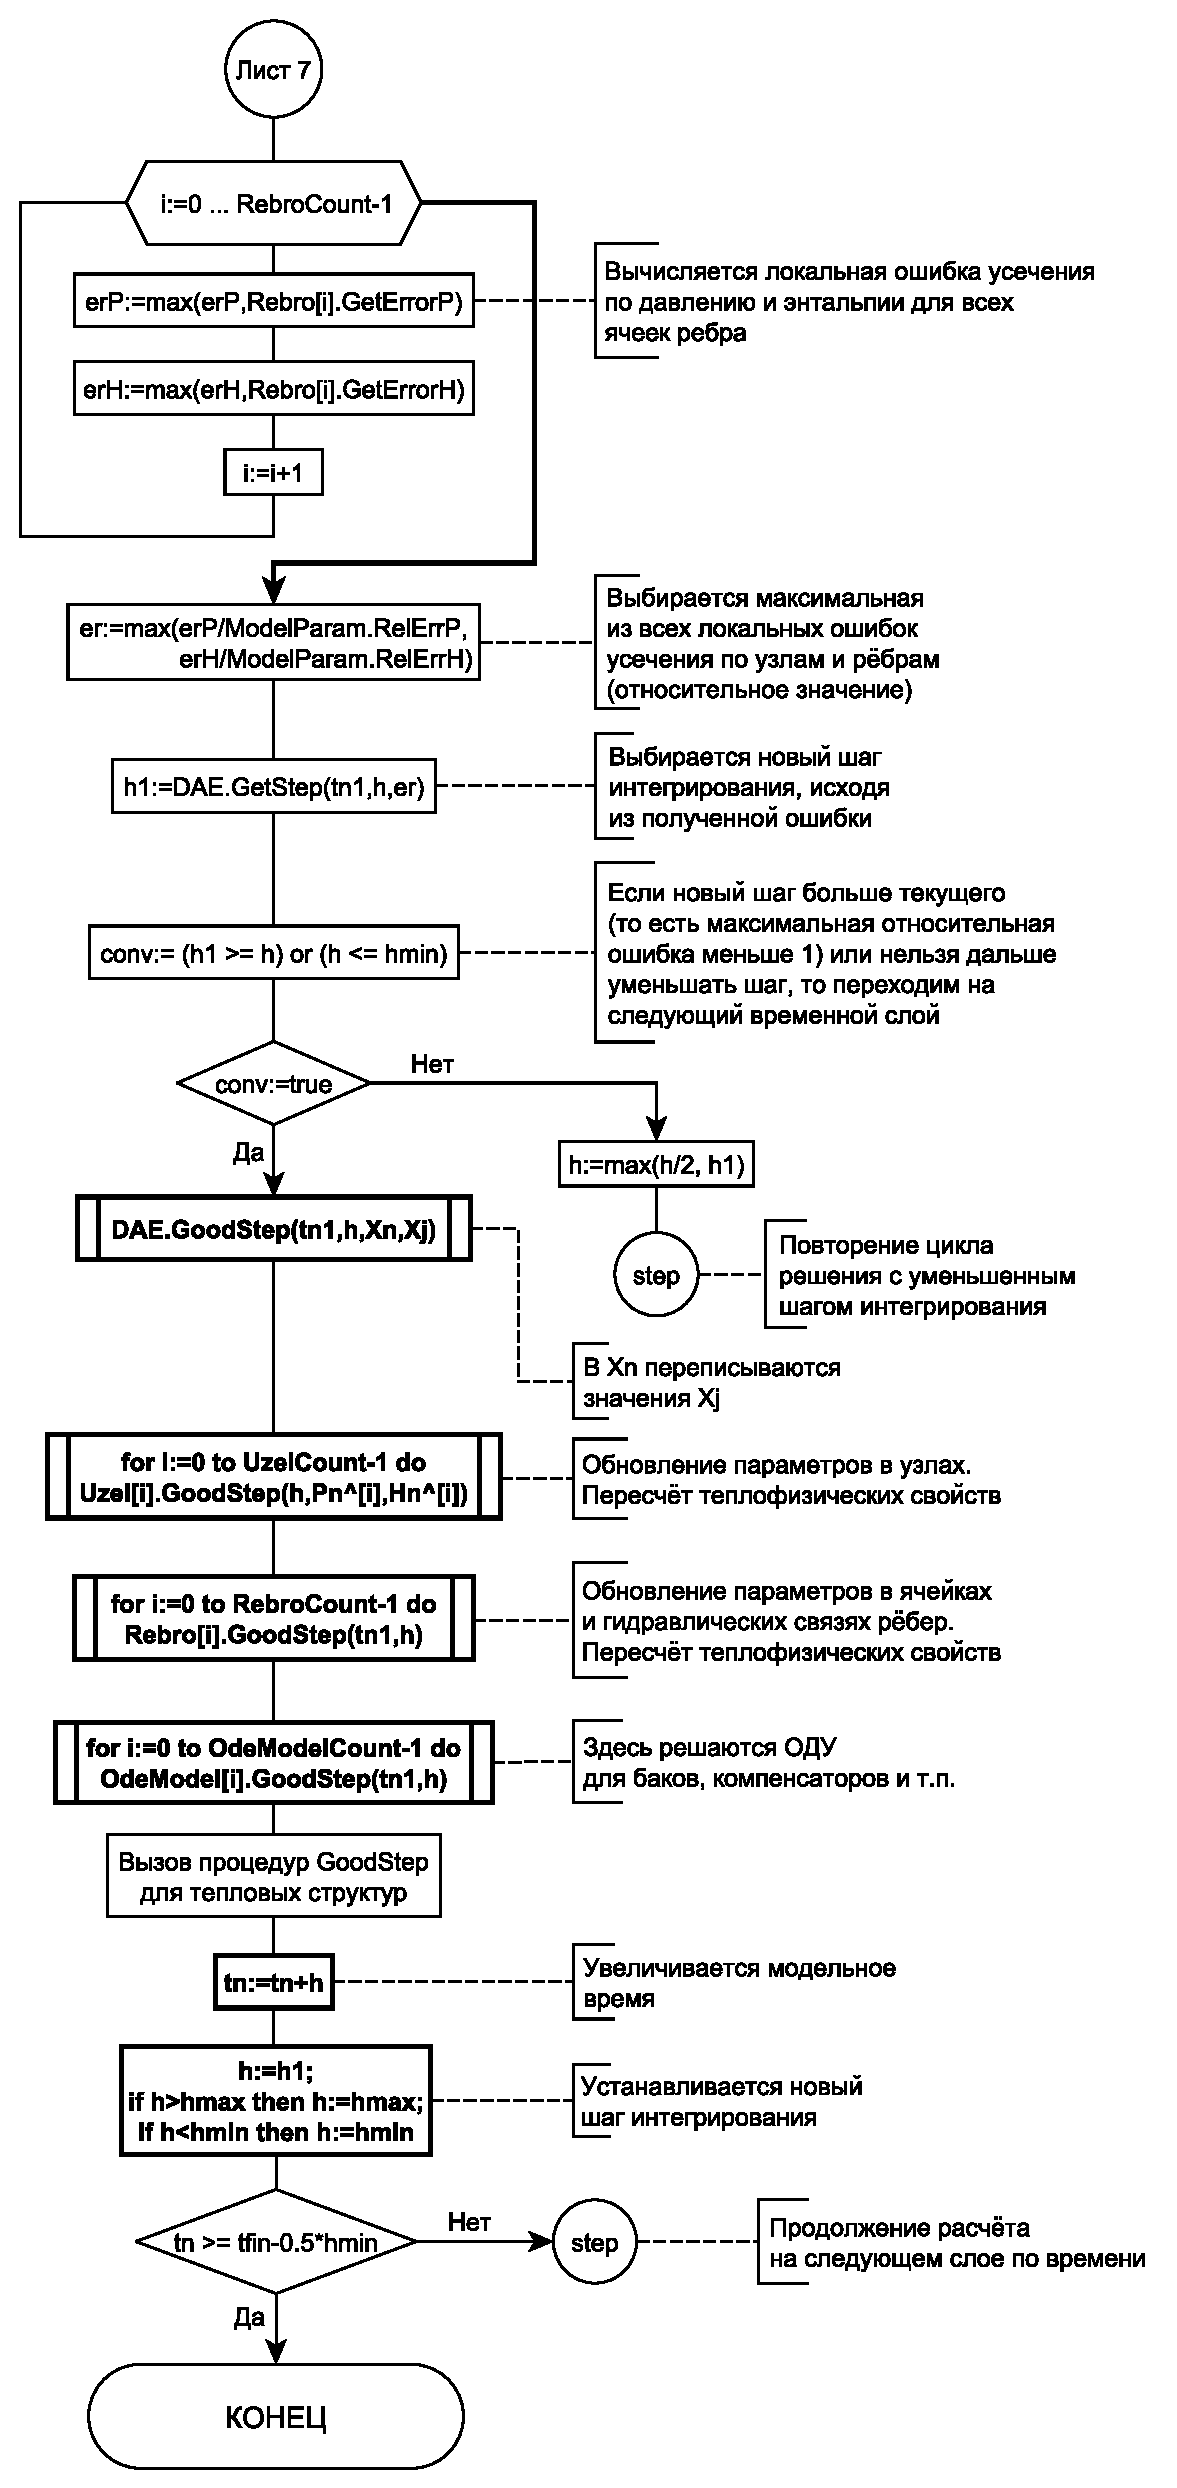
\includegraphics[width=0.69\linewidth]{Block_Scheme_Method1_List7.eps} 
	\caption{\textsc{Блок--схема алгоритма выполнения шага расчёта (лист 7)}}\label{fig97}
}
\end{figure}

\newpage




